\section{Introduction}\label{sec:intro}

\begin{figure}[t]
  \centering
  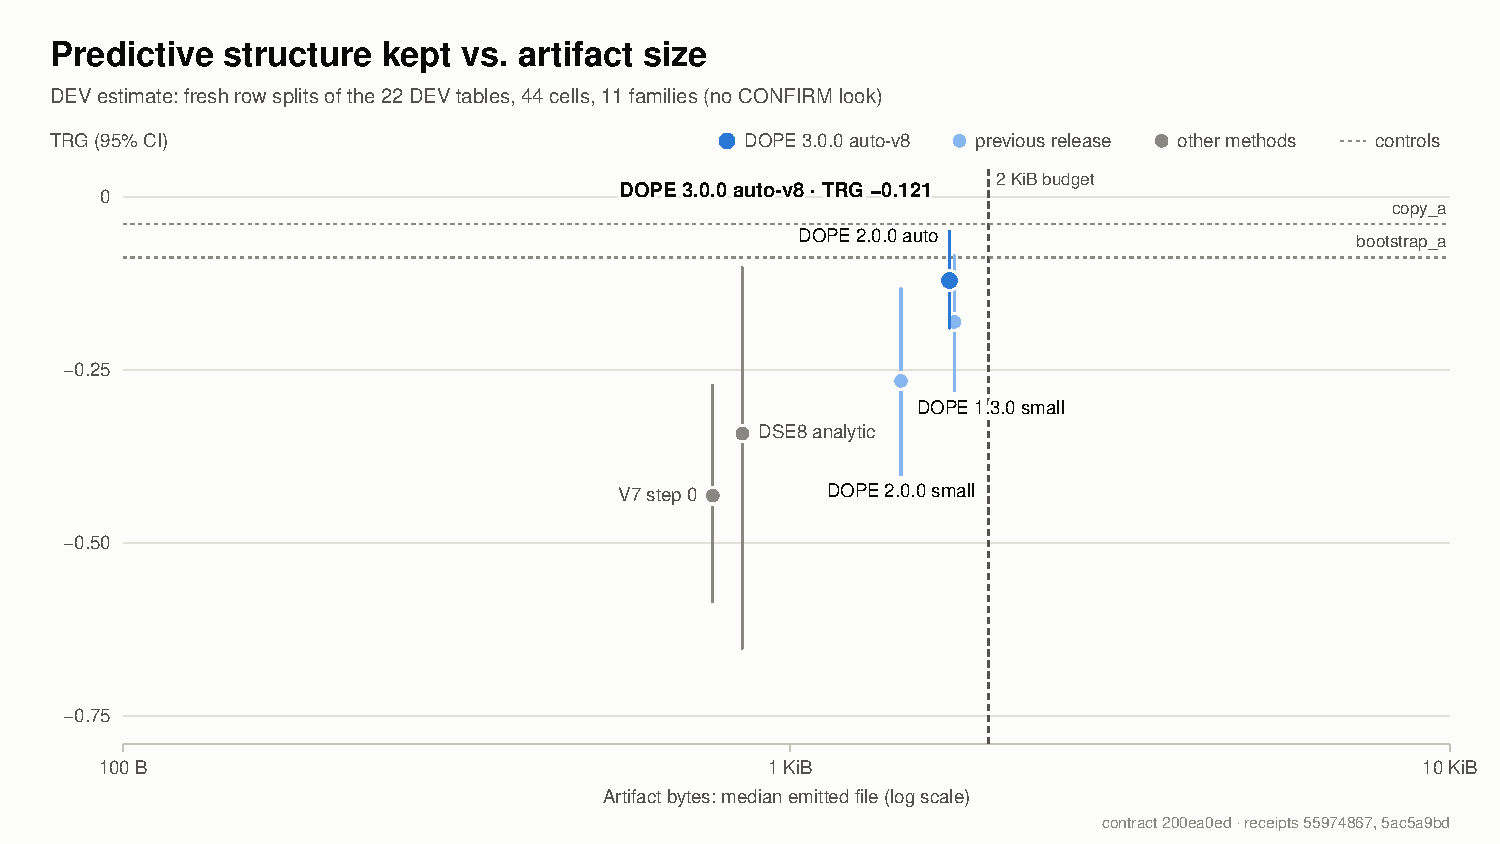
\includegraphics[width=\linewidth]{figures/hero-v3.pdf}
  \caption{TRG with its \VThree{CiLevel} family-bootstrap interval against the median file size (log axis) on the pre-registered report look (\S\ref{sec:protocol}): \VThree{CandCells} informative cells in \VThree{Families} families. The dashed line is the \VThree{BudgetBytes}-byte budget; dotted lines are the copy and bootstrap controls of $A$. This is the README figure, written by \texttt{dope\_kpi render-hero} from the receipts (SHA-256 prefixes \texttt{\VThree{PrimarySha}}, \texttt{\VThree{CompareSha}}) and converted to PDF without change (source SVG \texttt{\VThree{HeroSvgSha}}). The third-party generators are not in the README figure; Tables~\ref{tab:arms} and~\ref{tab:methods} report them.}
  \label{fig:hero}
\end{figure}

Much of the demand for synthetic tabular data is downstream: a model is trained on synthetic rows and then used on real ones.
DOPE treats this as a compression problem.
A table with a declared target is the input to a compiler; its output is an artifact of at most $B$ bytes that stores no source rows, and a sampler draws rows from the artifact alone.
The question each release answers is how much of the table's predictive structure survives at a fixed byte budget, measured by learners that never see the source rows during training.

Earlier releases offered two encoders under a common container: the Format~1 program~\citep{dope2026v1} and, in release~\VThree{BaseVersion}, a per-table choice between Format~1 and the V7 single-encoding packet~\citep{dope2026v2}.
Release~\VThree{ReleaseVersion} replaces the second candidate with \texttt{DSE8}, an analytic packet that needs no trained weights, and adds the encoder \cli{-{}-format auto-v8}, which chooses per table between Format~1 and \texttt{DSE8} with a duplicate-grouped two-fold check on the fitting rows.
The whole file, header included, stays within the budget (\VThree{BudgetBytes}~bytes by default).

\paragraph{Contributions.}
\begin{enumerate}
  \item \textbf{A packet codec with an explicit byte model} (\S\ref{sec:codec}, Appendix~\ref{app:codec}). \texttt{DSE8} is a CRC-checked sequence of tagged sections. Mandatory sections are sized by a closed-form byte model before fitting; optional sections are appended in a fixed order and truncated to the longest prefix that fits. Decoding is row-local and counter-seeded, so row $i$ depends only on the artifact, the seed and $i$.
  \item \textbf{An analytic, weight-free fit of that packet from the fitting rows only} (\S\ref{sec:fit}): typed marginals clipped at a support floor, a low-rank factor copula with regimes, and a calibrated target head with gated effects, pairwise interactions and oblivious trees.
  \item \textbf{Per-table codec selection} (\S\ref{sec:select}): \cli{auto-v8} keeps \texttt{DSE8} only when it beats Format~1 by a margin on a target-stratified, duplicate-grouped two-fold check and loses little on each fold.
  \item \textbf{A FIT-only evidence bank} (\S\ref{sec:evidence}): a deterministic, layout-frozen summary of the fitting rows that is invariant to row order and equivariant to column order, built to train learned encoders without per-table caching or access to evaluation rows.
  \item \textbf{A complete account of one pre-registered evaluation} (\S\S\ref{sec:protocol}--\ref{sec:results}), including the guards that fail, a sign-flip calibration of the decision rule and four third-party generators scored under the same protocol. Every number in this paper is rendered from committed receipts and checked in continuous integration (\S\ref{sec:repro}).
\end{enumerate}

\paragraph{What we do not claim.}
The evaluation is a development-set estimate; no confirmation, holdout or sealed panel was opened.
The comparison against the previous encoder improves TRG but its outcome under the contract is \VThree{Outcome}, not PROMOTE.
The artifacts do not make synthetic rows realistic in the two-sample sense, and the privacy diagnostics are empirical audits, not guarantees.
Section~\ref{sec:limits} lists these limitations in full.
